\documentclass[base.tex]{subfiles}
\begin{document}
\subparagraph{Plusieurs énoncé équivalents}
On va se servir systèmatiquement des bijections entre divers ensemble \underline{dénombrables} (c'est à dire ceux qui sont en bijection avec $\mathbb{N}$ \\
\\
Soit la fonction suivante
\[U(n,x) \: n,x \in \mathbb{N}\]
%n n'est pas le programme vu que Pn l'est %
avec $n$ programme et $x$ l'entrée du programme.
\[n \rightarrow p_n \]
puis on applique $p_n$ à $x$ ou $n \rightarrow p_n$ est une numération des programmes $p\in\mathbb{P}$ . $p_n$ est le programme numéroté $n$.

\paragraph{Problème de l'arrêt - bis }
Instance : $(n,x) \: n,x \in \mathbb{N}$\\
Question : La fonction $U(n,x)$ est-elle définie sur la paire $(n,x)$ ? (La fonction $U$ étant à priori partielle ).\\
Ce problème est indécidable .\\
La fonction $U(n,x)$ s'appelle fonction universelle. L'algorithme qui calcule la fonction $U(n,x)$ englobe tous les algorithmes qu'il soit .\\
\\
\textbf{John Von Neumann :} Un programme c'est aussi un type de donnée à part entière . On peut le mettre dans la mémoire de la machine et traiter comme une donnée .\\
\\
L'algorithme universel contient , comme sa partie intégrante , un compilateur. Encore un rappel : c'est à la fonction $U(n,x)$ que nous avons appliqué la diagonalisation :
\[h(n)=U(n,n)+1\]
Si on pouvait rendre la fonction $U$ totale alors on obtiendrai une contradiction. La fonction $h(n)$ serait
\begin{itemize}
\item calculable
\item totale ( si $U$ était totale)
\item différents par rapport à toutes les fonctions de $x$ obtenues en fixant $n$ dans $U(n,x)$
  
  \end{itemize}
Quant on fixe la valeur de $n$ à $0,1,2,3,...$ on obtient les fonctions d'une variable $x$
\[U(0,x),U(1,x),U(2,x),...\]
et dans cette suite il y a toutes les fonctions calculables d'une variable car on à numéroté par 0,1,2,... tout les programmes .\\
Nous avons une bijection entre $\mathbb{N}^2$ et $\mathbb{N}$ . On peut transformer toute fonction de deux variable en une fonction d'une variable. Par exemple , pour $U(n,x)$ : \\
\\
Soit $V(N)$ la fonction suivante (avec $N\in \mathbb{N}$):
\[N\rightarrow (n,x)\rightarrow U(n,x)\]
$(n,x)$ étant la paire numéro $N$\\
Fondamentalement , $V(N)$ c'est la même fonction que $U(n,x)$ . Les questions de calculabilités sont équivalentes.

\paragraph{Problème de l'arrêt - 3ème version}
Instance : un entier $N \in \mathbb{N}$\\
Question : la fonction $V$ est-elle définie au point $N$ ?\\
Ce problème est indécidable.\\
\\
Soit $q\in\mathbb{P}$ le programme qui calcule la fonction $V$\\
Instance : un entier $N \in \mathbb{N}$\\
Question : $q$ appliqué à $N$ s'arrête t'il ?\\
Ce nouveau problème est lui aussi indécidable .\\
\\
Une conclusion technique très utile : il n'y a pas de différence fondamentales entre les fonctions de 1 ou de 2 , ou de 3 , ...,variables .
\[(t1,t2,t3)\Leftrightarrow N \Leftrightarrow (x_1,x_2,x_3,x_4,x_5)\]
Les relations entre des fontions calculables et les programmes qui les calculent sont non triviales . La même fonction peut être calculé par plusieurs programmes différents .\\
\\
%voir feuille 1 , tant que , retourner
\textbf{Rappel} \\
L'ensemble de toutes les fonctions $\mathbb{N}\rightarrow\mathbb{N}$ n'est pas dénombrables tandis que l'ensemble $\mathbb{P}$ des programmes est dénombrables.\\
Soit $\mathbb{H}$ l'ensemble des fonction $\mathbb{N}\rightarrow\mathbb{N}$ calculables ( on admet aussi les fonctions partiellements calculables). Pour toute fonction appartenant à $\mathbb{H}$ il existe un programme qui la calcule , et même plusieurs programmes .\\
\\
Supposon que $\mathbb{H}$ est subdivisée en 2 parties disjointes et non vides :
\[\mathbb{H}=\mathbb{A}\cup \mathbb{B}\]
\[\mathbb{A}\cup \mathbb{B} = \emptyset\]
\[\mathbb{A},\mathbb{B} \neq \emptyset\]
\subparagraph{Problème}
Instance : un programme $p\in \mathbb{P} $
\\
\textbf{Question} : Le programme $p$ calcule t'il une fonction appartenant à $\mathbb{A}$ ou à $\mathbb{B}$
%exemple de séparation feuille 2
\subsection{Théorème de rice} %XXX%
Quelque soit les ensemble $\mathbb{A}$ et $\mathbb{B}$ , le problème en question est toujours indécidable !

      \begin{figure}[!h]
         \centering
         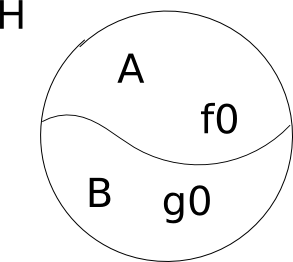
\includegraphics[scale=0.3]{rice}
      \end{figure}

Supposon qu'il existe un algorithme $R$ qui répond par oui ou ar non si un programme donnée $p$ calcule une fonction de $\mathbb{A}$ ou de $\mathbb{B}$ .\\
Alors considérons le programme $t$ suivant :
\[x\rightarrow t\]
\begin{itemize}
\item Appliquer l'algorithme $R$ à lui même
\item Si la réponse est oui retourner $q_0(x)$
\item Si la réponse est non retourner $p_0(x)$
\end{itemize}
$t$ calcule t'il une solution de $\mathbb{A}$ ou de $\mathbb{B}$ ?\\
Si de $\mathbb{A}$ alors de $\mathbb{B}$, et inversement.\\
\\
Symbole pour contradiction :
%pas encore trouvé dans latex$
\\
\\
L'algorithme $R$ est appliqué à lui même et c'est une forme de diagonalisation.
\[U(n,n)\]
avant n et n était des entiers .\\
$U(p,n)$ : Programme $p$ appliqué à $n$\\
$U(p,p)$ : Programme $p$ appliqué à lui même \\
$U(n,n)$ puis changer , par exemple $U(n,n)+1$

\subsection{Ensemble décidables et semi-décidables}
On choisi d'abord un "univers" $\Omega :\mathbb{N},\mathbb{N}^2,\sum^*,\mathbb{P},\{graphes\},...$\\
\\
\textbf{Définition 1:} Un ensemble $X\subseteq \Omega$ est décidable s'il existe un algorithme qui , pour un $x \in \Omega$ donnée , répond par oui ou par non si $x \in X$ ou non .\\
\\
\textbf{Définition 2:} Un ensemble $X\subseteq \Omega$ est semi-décidable s'il existe un algorithme qui , pour un $x\in \Omega$ donnée , répond oui si $x \in X$.
\\
\\
Prenons $\Omega = \mathbb{N}$\\
L'ensemble des parties de $\mathbb{N}$ n'est pas dénombrable . Par conséquent , la pluparts des parties de $\mathbb{N}$ ne sont ni décidable , ni semi décidable. \\
Mais peut-t'on donné un exemple concret ?\\
Ex : L'ensemble $\{(p,x)|p \in \mathbb{P} , x \in \mathbb{N} : p$ s'arrête sur $x\}$ est semi décidable mais pas décidable .\\
Semi-décidabilité : appliqué $p$ à $x$ et attendre.

\end{document}
